\documentclass[journal]{vgtc}                % final (journal style)
% \documentclass[review,journal]{vgtc}         % review (journal style)
%\documentclass[widereview]{vgtc}             % wide-spaced review
%\documentclass[preprint,journal]{vgtc}       % preprint (journal style)

%% Uncomment one of the lines above depending on where your paper is
%% in the conference process. ``review'' and ``widereview'' are for review
%% submission, ``preprint'' is for pre-publication, and the final version
%% doesn't use a specific qualifier.

%% Please use one of the ``review'' options in combination with the
%% assigned online id (see below) ONLY if your paper uses a double blind
%% review process. Some conferences, like IEEE Vis and InfoVis, have NOT
%% in the past.

%% Please use the ``preprint''  option when producing a preprint version
%% for sharing your article on an open access repository

%% Please note that the use of figures other than the optional teaser is not permitted on the first page
%% of the journal version.  Figures should begin on the second page and be
%% in CMYK or Grey scale format, otherwise, colour shifting may occur
%% during the printing process.  Papers submitted with figures other than the optional teaser on the
%% first page will be refused. Also, the teaser figure should only have the
%% width of the abstract as the template enforces it.

%% These few lines make a distinction between latex and pdflatex calls and they
%% bring in essential packages for graphics and font handling.
%% Note that due to the \DeclareGraphicsExtensions{} call it is no longer necessary
%% to provide the the path and extension of a graphics file:
%% 
\includegraphics{diamondrule} is completely sufficient.
%%
\ifpdf%                                % if we use pdflatex
  \pdfoutput=1\relax                   % create PDFs from pdfLaTeX
  \pdfcompresslevel=9                  % PDF Compression
  \pdfoptionpdfminorversion=7          % create PDF 1.7
  \ExecuteOptions{pdftex}
  \usepackage{graphicx}                % allow us to embed graphics files
  \DeclareGraphicsExtensions{.pdf,.png,.jpg,.jpeg} % for pdflatex we expect .pdf, .png, or .jpg files
\else%                                 % else we use pure latex
  \ExecuteOptions{dvips}
  \usepackage{graphicx}                % allow us to embed graphics files
  \DeclareGraphicsExtensions{.eps}     % for pure latex we expect eps files
\fi%

%% it is recomended to use ``\autoref{sec:bla}'' instead of ``Fig.~\ref{sec:bla}''
\graphicspath{{figures/}{pictures/}{images/}{./}} % where to search for the images

\usepackage{microtype}                 % use micro-typography (slightly more compact, better to read)
\PassOptionsToPackage{warn}{textcomp}  % to address font issues with \textrightarrow
\usepackage{textcomp}                  % use better special symbols
\usepackage{mathptmx}                  % use matching math font
\usepackage{times}                     % we use Times as the main font
\renewcommand*\ttdefault{txtt}         % a nicer typewriter font
\usepackage{cite}                      % needed to automatically sort the references
\usepackage{tabu}                      % only used for the table example
\usepackage{booktabs}                  % only used for the table example
%% We encourage the use of mathptmx for consistent usage of times font
%% throughout the proceedings. However, if you encounter conflicts
%% with other math-related packages, you may want to disable it.

%% In preprint mode you may define your own headline. If not, the default IEEE copyright message will appear in preprint mode.
%\preprinttext{To appear in IEEE Transactions on Visualization and Computer Graphics.}

%% In preprint mode, this adds a link to the version of the paper on IEEEXplore
%% Uncomment this line when you produce a preprint version of the article 
%% after the article receives a DOI for the paper from IEEE
%\ieeedoi{xx.xxxx/TVCG.201x.xxxxxxx}

%% If you are submitting a paper to a conference for review with a double
%% blind reviewing process, please replace the value ``0'' below with your
%% OnlineID. Otherwise, you may safely leave it at ``0''.
\onlineid{0}

%% declare the category of your paper, only shown in review mode
\vgtccategory{Research}
%% please declare the paper type of your paper to help reviewers, only shown in review mode
%% choices:
%% * algorithm/technique
%% * application/design study
%% * evaluation
%% * system
%% * theory/model
\vgtcpapertype{please specify}

%% Paper title.
\title{AsylumLoupe: EU Asylum Demographics and Movement Information Visualization}

%% This is how authors are specified in the journal style

%% indicate IEEE Member or Student Member in form indicated below
\author{Han Wang and Xin Wang}
\authorfooter{
%% insert punctuation at end of each item

\item 
 All authors contributed equally to this work.
\item
 Han Wang, E-mail: whan2019@student.ubc.ca.
\item
 Xin Wang, E-mail: wangxin0@student.ubc.ca.
}

%other entries to be set up for journal
% \shortauthortitle{Biv \MakeLowercase{\textit{et al.}}: Global Illumination for Fun and Profit}
%\shortauthortitle{Firstauthor \MakeLowercase{\textit{et al.}}: Paper Title}

%% Abstract section.
\abstract{write abstruct here!} 
% end of abstract

%% Keywords that describe your work. Will show as 'Index Terms' in journal
%% please capitalize first letter and insert punctuation after last keyword
\keywords{Asylum, EU, Refugees, Information Visualization}

%% ACM Computing Classification System (CCS). 
%% See <http://www.acm.org/class/1998/> for details.
%% The ``\CCScat'' command takes four arguments.

% \CCScatlist{ % not used in journal version
%  \CCScat{K.6.1}{Management of Computing and Information Systems}%
% {Project and People Management}{Life Cycle};
%  \CCScat{K.7.m}{The Computing Profession}{Miscellaneous}{Ethics}
% }

%% Uncomment below to include a teaser figure.
\teaser{
  \centering
  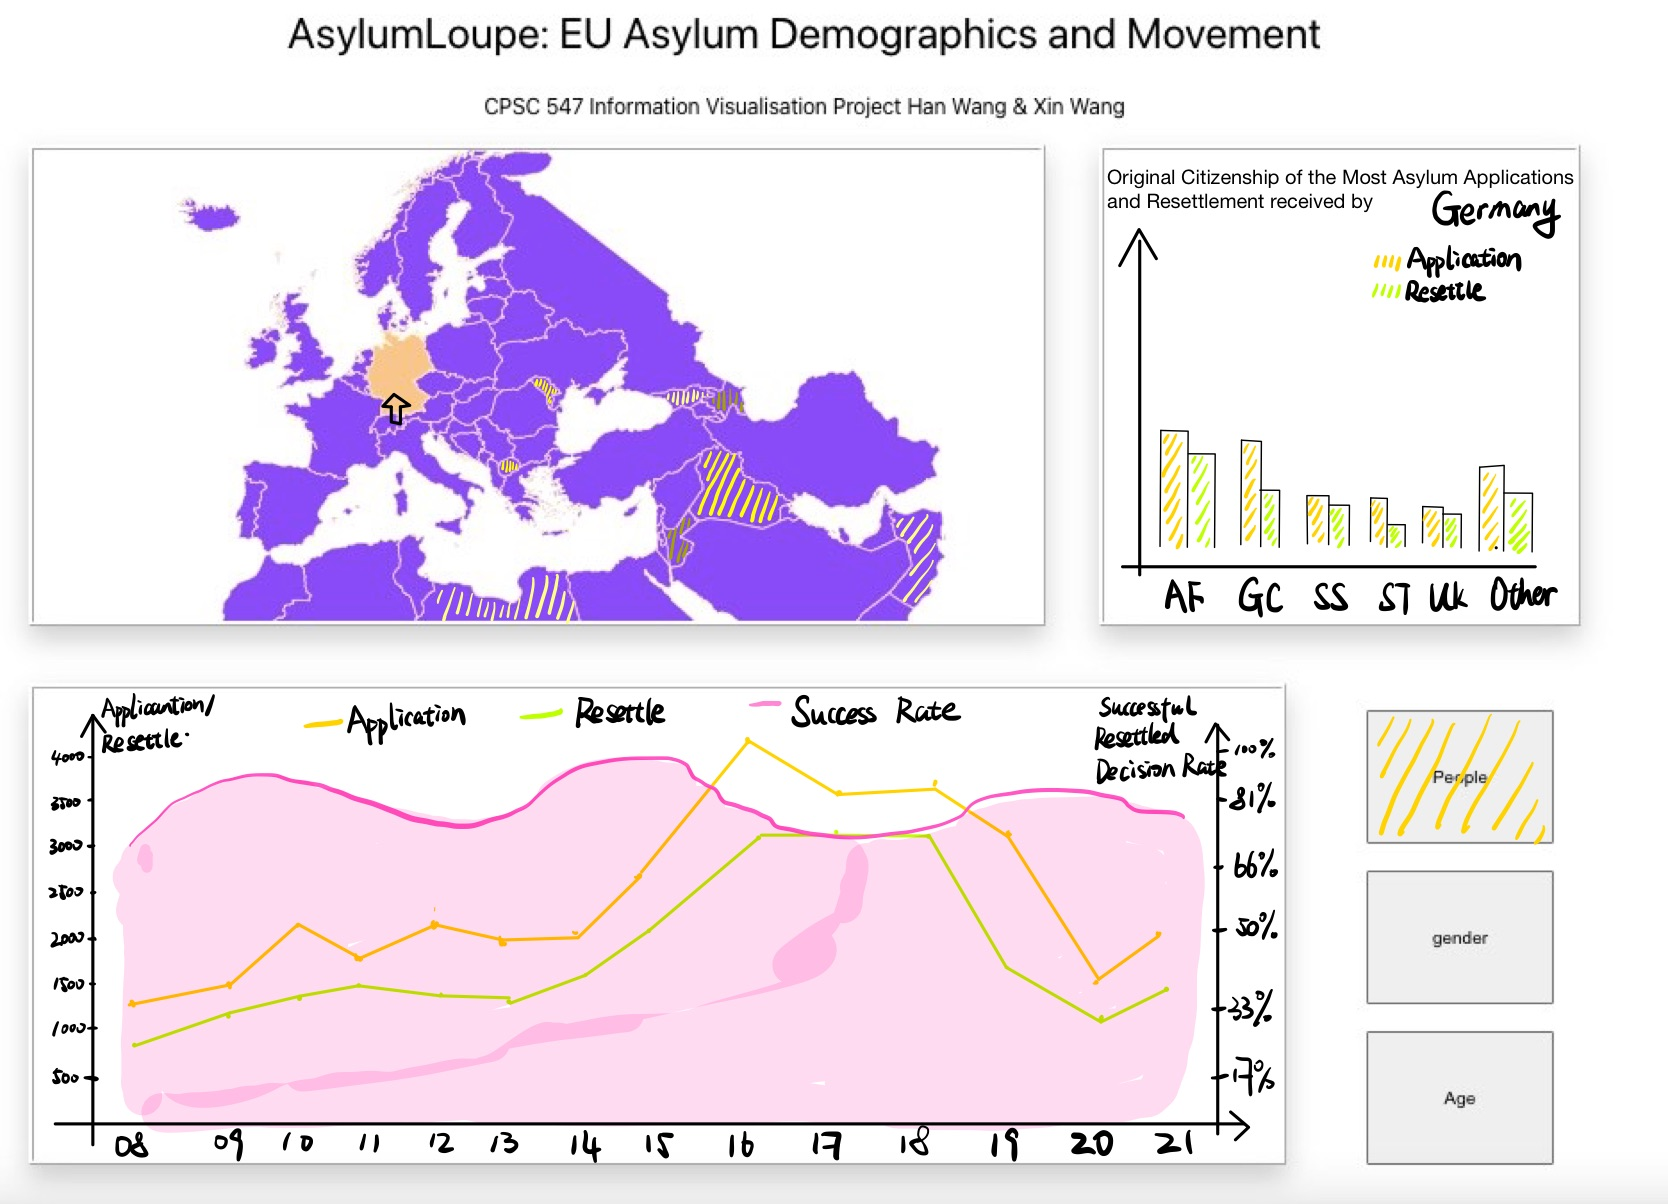
\includegraphics[width=\linewidth]{Sketches-1}
  \caption{AsylumLoupe interface, showing incoming asylum applicants and resettlement receivers in Germany between 2008 and 2022.}
	\label{fig:teaser}
}

%% Uncomment below to disable the manuscript note
\renewcommand{\manuscriptnotetxt}{}

%% Copyright space is enabled by default as required by guidelines.
%% It is disabled by the 'review' option or via the following command: \nocopyrightspace

\vgtcinsertpkg
\nocopyrightspace
%%%%%%%%%%%%%%%%%%%%%%%%%%%%%%%%%%%%%%%%%%%%%%%%%%%%%%%%%%%%%%%%
%%%%%%%%%%%%%%%%%%%%%% START OF THE PAPER %%%%%%%%%%%%%%%%%%%%%%
%%%%%%%%%%%%%%%%%%%%%%%%%%%%%%%%%%%%%%%%%%%%%%%%%%%%%%%%%%%%%%%%%

\begin{document}

%% The ``\maketitle'' command must be the first command after the
%% ``\begin{document}'' command. It prepares and prints the title block.

%% the only exception to this rule is the \firstsection command
\firstsection{Introduction}

\maketitle

%% \section{Introduction} %for journal use above \firstsection{..} instead
The war in the Middle East, the oil crisis, and geopolitical issues have all caused many people to be displaced. Despite continued COVID-19 measures, the number of arrivals to Europe's external borders increased in 2021, returning to pre-pandemic levels. Adapting quickly, EU+ countries (the European Union, Israel, Norway, Serbia, Turkey, and the United Kingdom) facilitated asylum application lodgings, rearranged reception facilities, and used arrival centers for various stages of asylum procedures in response to the waves of arrivals\cite{euaa:2022}. These developments have also highlighted the need for structural reforms of the EU's asylum and migration system to address both crises and longer-term trends\cite{hurwitz:2009}. The existing asylum procedure has been developed from each stage, and the process has been digitized recently as well, including procedures for first and second applications, special procedures, the Dublin procedure, reception conditions, detention during the asylum procedure, access to the asylum procedure and information, legal assistance, interpretation services, country of origin information, the content of protection, the return of former applicants and resettlement. The Dublin procedure establishes the criteria to determine which Member State is responsible for examining an application for international protection. It is a Europe-wide procedure that follows the same criterion for determining responsibility applied similarly in all Member States. There are differences in national legislation and organizational set-ups of Member States, which is why diverse national practices exist when applying the regulation. 

Identifying and monitoring trends in asylum applicants and country of origin countries can be accomplished through the key indicators presented\cite{euaa:2022}. The EU has always been welcoming to refugees, and even before the 2015 refugee crisis, the EU asked its members to submit a series of refugee-related data, which can be found on the Eurostat, which is the statistical database of the European Union to provide high-quality statistics and data on Europe. This database details the number of refugee applicants, temporary asylum seekers, and long-term asylum seekers by age, gender, and nationality since 2008. The European Council committed in 1999 to develop a Common European Asylum System (CEAS) that applies the Geneva Convention fully and inclusively. For the CEAS to develop in the right direction, a period of reflection was required after the first phase. There were still too many differences across EU Member States, and protection levels were still insufficient. As a result of this, the European Commission presented its Asylum Policy Plan in June 2008, which laid the foundation for a system of common and uniform protection standards. In that case, we will use this data from 2008 to 2021 to develop Vis to show and analyze many issues. 

The primary objective of this project is to provide an overview of the refugee intake trends across 27 EU member countries. We also want to present the different distribution of asylum applications, temporary asylum, and long-term asylum across EU member states, and the differences between countries of origin, gender, and age of asylum seekers as detailed information. In that case, we propose an explorer tool to support users to figure out the refugee movement trends within the EU as time progresses. It should also be a helpful analysis tool for users to acquire detailed and intuitive information introduced above and compare them by specific years.

To facilitate better planning resources for future asylum seekers, this project may provide a more intuitive and easier way for a user working for specific institutions to explore the movement of asylum applicants compared to searching and analyzing huge amounts of data from data tables and trees layer by layer the detailed explanation will be described in section 3, Data and Task Abstraction.

\section{Related Work}
\subsection{Asylum in Europe and Asylum Demographic Data}
Asylum refers to the international protection offered by a country on its territory. It is provided for people who cannot seek protection in their own country of citizenship and/or residence, especially those who fear persecution based on race, religion, nationality, wars, membership in a particular social group, or political opinion\cite{unhcr:2012}. This paper presents a information visualization (Vis) project concerning asylum seekers and resettlement in the European Union. Processing asylum applications and resettlement is covered by the EU migration policy. The EU has a long history of regulating its immigration policy, and since the 1951 Convention Relating to the Status of Refugees\cite{the_european_commission:2022}, the EU has continued to improve its migration policy, establishing the current harmonized legislative framework on asylum based on the Treaty on the Functioning of the European Union and the EU Charter of Fundamental Rights as its legal foundation. Each year, the EU makes effort to develop an effective European migration and asylum policy in response to large numbers of migrants coming to the EU resulting from migration crises like the one in 2015\cite{consilium:2022}. The creation of a migration and asylum policy and its operation is based on collecting data on the current situation. An example is the demographic data related to asylum application and resettlement in the EU discussed in this project. 

Eurostat (European Statistical Office), which provides statistical information to the institutions of the European Union, persists datasets related to EU asylum application and resettlement. In terms of presenting these data, Eurostat used a range of published charts with pre-defined data types derived from the dataset of asylum demographics. Eurostat provides a data visualization tool that is integrated into its powerful Eurostat Data Browser\cite{data_browser_eurostat:2020}. For each new dataset published, Eurostat presents the data in the Vis idioms of tables, graphs, and maps on its web page. The Eurostat also integrates the Data Explorer tool, a feature that presents the charts as a search tree. Users can click on a search tree branch to display different charts. While supporting the functionality that current tool provided, the new data browser also adds additional functionality for viewing data and metadata: users can filter data dimensions and adjust the way graphical data is displayed (line, bar, and map charts), which makes it easy to compare indicators and geographical areas\cite{wiki_eurostat:2022}. 
\subsection{Information Visualization Design}
We want to build Vis idioms showing the demographics and movements of asylum application and resettlement in the EU. We need to represent the movement of asylum applicants and resettled refugees by showing the association between known geographic pairs, such as refugees drifting from a country at war, to an EU country seeking asylum. The O(Origin)D(Destination) Map is a good solution for this. OD Map shows the relationship by mapping the geographic vectors between the origin and destination as cells rather than lines. It preserves the spatial layout of OD, and when we need to show multiple “origins” of the “destination” country, e.g., an EU country receiving asylum applications from people in multiple countries, the OD Map does not suffer from the occlusion problems of other solutions, or the loss of detail due to aggregation\cite{slingsby:2010}. Choropleth map utilizes the color channel in corresponding to an aggregated summary of geographic characteristics within spatial enumeration units\cite{dent:1990}, it can visualize how an attribute from our dataset varies across the geographic area. In our case, the choropleth map can contribute to showing the different magnitudes of an attribute in our dataset encoded by saturation and the color channel. Stacked bar charts can help us make more complex data comparisons. A stacked bar chart is a form of bar chart that follows the horizontal coordinates to show the composition and comparison of multiple variables. After selecting the source and destination countries, our Vis will provide comparisons of demographic data, such as comparisons of asylum application, and resettlement numbers by gender, age group, and other ordinal or categorical characteristics. Stacked bar charts allow us to show how these comparisons have changed over time\cite{donnelly_kelley:2013}.

\section{Data and Task Abstraction}

\subsection{Domain}

This Vis project focuses on illustrating the movement and analyzing the demographic data of asylum application and resettlement across Europe, the Middle East, and North Africa (MENA) region from 2008 to 2021. We want to combine credible and rich data in an interactive format to dynamically show the movement of  asylum applicants and resettled refugees in the same time period. Based on this, we will also explore different trends in combination with their demographic data. Our project helps EU policymakers to understand the movement of asylum applicants, explore the changing trends of asylum seekers’ demographic over time, and develop corresponding policies on asylum seekers or refugees, predict the future increase or decrease of asylum seekers in the EU. People in each EU country can also use our project to learn about the asylum demographics in their own country, such as age, gender and original nationality. Therefore, they can learn about domestic asylum with real data, which helps society to eliminate prejudice against asylum receivers and refugees. 

\subsection{Tasks Abstraction}

The biggest task of this project in terms of Vis is to show the movement of asylum applicants,  and resettled refugees in the Europe and MENA region from 2008 to 2021, including their countries of origin and destination. Users can explore the correlation and distribution of asylum applicants and resettled refugees with different age classes, gender classes, and original nationalities across the EU countries. They can also compare the asylum application intake and resettled decisions of the applicants between each year from 2008 to 2021, and find the correlation between successful resettled decisions for asylum applications and different EU countries. On top of this, the project will also select associations between origin countries and  one EU country that has asylum application or resettlement intake. In the case of both origin and destination countries are selected, the distribution of age class, gender class, and original nationality will be presented to allow the reader to identify different patterns and trends. The user can specify different attributes to observe the distribution of these attributes in different classes from 2008 to 2015 and explore the correlation between attributes like age or gender classes and the successful resettled decision in each year.

\subsection{Data Abstraction}
Data for this project are sourced from Eurostat. We selected the annual aggregated data series on asylum applications and resettlement containing statistical information based on Article 4 of the Council Regulation (EC) No 862/2007 from 2008 to 2021. We didn’t adapt the historic data before 2008. The Council Regulation (EC) No 862/2007 concluded the regulation for collecting and analyzing information on migration and asylum in the EU, which included several important changes designed to improve the completeness and degree of harmonization of these statistics\cite{eur_law:2007}. To avoid massive inconsistent data entries, we only sample the dataset referencing this regulation starting from 2008.

Our final dataset will be obtained by concatenating 2 related datasets, the dataset for asylum applicants in all EU member countries and resettlement decision in all member countries from 2008 to 2015. As of today, we worked with more than 1,000,000 items. Each item represents the status of one asylum application or resettlement with reference to different age classes, gender classes, and original citizenship. The national Ministries of Interior and related official agencies provide these data to Eurostat. Data is presented by country and for groups of countries: the European Member States and the European Free Trade Association (EFTA). The attributes we intend to use in our analysis are both categorical and ordered. Dataset is constantly updated\cite{european_commission:2021}. We selected the newest latest dataset on 13th November 2022. Specifically, the levels of categorical attributes are as shown in \autoref{tab:lev1}. The ranges for ordered attributes are listed in \autoref{tab:lev2}. One example item/data entry from the origin datasets is presented in the \autoref{fig:tab3}.

\begin{table}[tb]
  \caption{Level of Categorical Attributes for EU Asylum Application and Resettlement Dataset - Annual Aggregated Data}
  \label{tab:lev1}
  \scriptsize
	\centering
  \begin{tabular}{p{0.2\linewidth}p{0.1\linewidth}p{0.2\linewidth}p{0.3\linewidth}}
    \toprule
    Dimensions[code] & Levels & Labels[code] & Note \\
    \midrule
    Time-Frequency [FREQ] & 1 & Annual[A] & Only annual data included \\
    Country-of-Citizenship [CITIZEN] & 208 & Countries, or regions defined by Eurostat represent by ISO 3166-1 alpha-2 country codes. & We cleaned the data, only Europe and MENA countries and regions remain in final dataset. \\
    Sex [SEX] & 4 & Total [T], Males [M], Females [F], Unknown [UNK] & [T] equals the sum of [M], [F] and [UNK]. \\
    Application-Type [asyl\_app] & 3 & Asylum-Applicant [ASY\_APP], First-Time-Applicant [NASY\_APP], Subsequent-Applicant [SSEQ] & [ASY\_APP] equals [NASY\_APP] plus [SSEQ], asylum application dataset only. \\
    Unit of Measure [unit] & 1 & Person [PER] & \\
    Geopolitical Entity [geo] & 34 & 33 geo political entities in EU plus European Union of 27 member states [EU27\_2020] & Geo political entities include the EU, EEA(European Economic Area), EFTA countries, exit members included.
  \end{tabular}
\end{table}

\begin{table}[tb]
  \caption{Range of Ordered Attributes for EU Asylum Application and Resettlement Dataset - Annual Aggregated Data}
  \label{tab:lev2}
  \scriptsize
	\centering
  \begin{tabular}{p{0.2\linewidth}p{0.35\linewidth}p{0.35\linewidth}}
    \toprule
    Dimensions[code] & Range[code] & Note \\
    \midrule
    Age Class [Age] & Total [Total], Less than 14 [Y\_LT14], From 14 to 17 [Y14-17], Less than 18 [Y\_LT18], From 18 to 34 [Y18-34], From 35 to 64 [Y35-64], 65 or older [Y\_GE65], Unknown [UNK] & Age of the applicants are distributed into 8 classes, some countries didn't split the class under 18. \\
    Time [Time] & From 2008 to 2021 & Each year represents an attribute. \\
    Cell value & From 0 to 1216806 & Value of each year, represents the number of applications or resettlements. \\
  \end{tabular}
\end{table}

\begin{figure}[tb]
  \centering % avoid the use of \begin{center}...\end{center} and use \centering instead (more compact)
  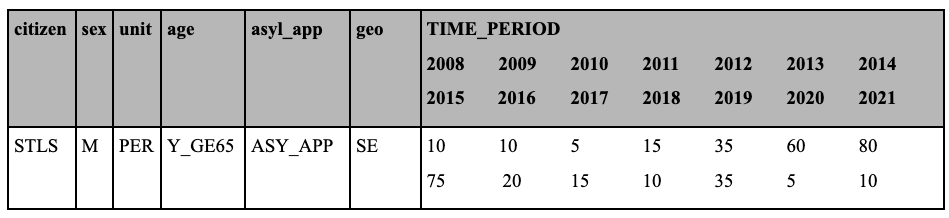
\includegraphics[width=\columnwidth]{tab3.png}
  \caption{Example Data Entry for EU Asylum Application Dataset - Annual Aggregated Data}
  \label{fig:tab3}
 \end{figure}

We filtered out the “Time of Frequency” and “Unit of Measure” attributes, which have the same value in each entry and contain no additional information. We also filter out certain levels or ranges for the different attributes, and the specific information is summarized in the note column on the right of each table. We cleaned the data before implementing the Vis. We used Numpy and pandas libraries in python to eliminate all non-compliant attributes. In the original data, all “Time” attributes were listed in one column, and we separated the “Time” attributes by commas so that each different class of Time was given a separate column. We then align it with other data in the same row to get a valid CSV file. Next, we tackled the non-compliant values, e.g. some of the “Time” attributes have non-integer data in the field, which we change to 0. We use the summation formula to sum the values of all the time attributes of each entry when the value sum of all time attributes is 0, it proves that there is no record of this type of application or resettlement entry, so we also eliminate it. After finishing the data cleaning, we have 87,728 rows of application data and 6908 rows of resettlement data left. \autoref{fig:tab4} lists the sample rows of application/resettlement after completing the cleaning.

\begin{figure}[tb]
  \centering % avoid the use of \begin{center}...\end{center} and use \centering instead (more compact)
  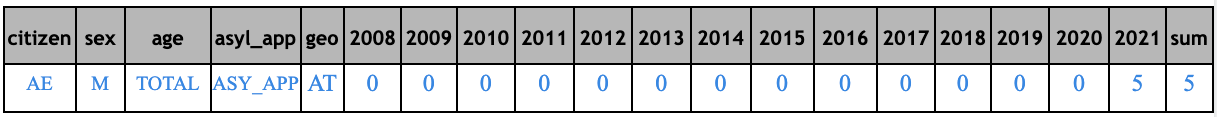
\includegraphics[width=\columnwidth]{tab4.png}
  \caption{Example Cleaned Data Entry for EU Asylum Application Dataset - Annual Aggregated Data}
  \label{fig:tab4}
 \end{figure}

\section{Solution}

This section depicts the potential scenarios for this project and the possible solutions associated with them. The scenarios and solutions will be introduced from two aspects, overview and detail. We will use React.js along with D3.js to implement the visualization and interaction functions. We will acquire data directly from local CSV files which are preprocessed by data cleaning. We will also use redux to enhance the interaction speed if it is needed. We aim to host our visualization tool on a website that can be easily accessed by prospective users.

\subsection{User Scenario 1}
\subsubsection{Senario Solution}
For the destination countries, which are EU+ countries, where refugee asylum claims are processed, refugee service agencies would like to assess whether basic services such as infrastructure, service personnel, and service types need to be improved by analyzing specific data in a certain year since EU+ countries aim to provide continuously improved services for asylum seekers. The first user scenario is that EU+ countries handle asylum applications and make decisions on resettlement. For example, analyzing and improving the configuration of the number of different language service providers based on the asylum application data flowing into the destination country through the visualized data in the view. Another example is to increase or decrease the infrastructure required for a specific age group through the asylum application age visualization displayed in the view.

Using data visualization, this project assists refugee service agencies in better intuitively analyzing how to improve their configuration and infrastructure. For example, analyzing and improving the configuration of the number of different language service providers based on the asylum application data flowing into the destination country through the visualized data in the view. Another example is to increase or decrease the infrastructure required for a specific age group through the asylum application age visualization displayed in the view.

As shown in \autoref{fig:us1-1}, The immigration officer from one EU+ country, for instance, Germany wants to compare the asylum statistic between 2008 and 2021 to explore the correlation between asylum applicants and their original citizenship. Along with time progress, the officer wants to know people from which countries or regions sent the most asylum applications to Germany and from which country or regions have the highest possibility to receive a resettled decision. The officer could also compare the total number of asylum applicants and resettlement between different years, if a growing trend is explored, the officer could allocate more resources to asylum matters or call for help from other member states.

\begin{figure}[tb]
  \centering % avoid the use of \begin{center}...\end{center} and use \centering instead (more compact)
  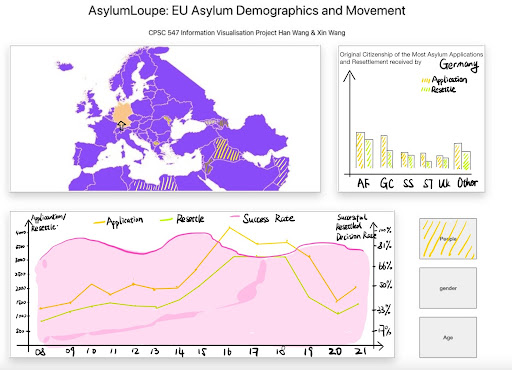
\includegraphics[width=\columnwidth]{fig2}
  \caption{Project Overview Schematic Diagram under User Scenario 1}
  \label{fig:us1-1}
 \end{figure}

For example, the picture above depicts the example mentioned before. After clicking the region of Germany, the German immigration officer will get further information about the origin countries asylum seekers come from. The view at the top-right corner shows the statistical asylum data in Germany from different origin countries asylum seekers come from. Since the button “people” is chosen, this view shows the visualization of the data of asylum applications and resettlement processed in Germany in a bar chart format. The view below represents the statistical asylum application and resettlement data in Germany from 2008 to 2021 in a line chart format, and the level of quantity is measured by the left axis. In this way, the German immigration officer can judge decisions like whether it is necessary to expand refugee shelters based on the trend of the number of asylum applications flowing from the origin country to Germany or judge whether the efficiency of the asylum application processing period needs to be improved based on the trend of the success rate of the number of asylum applications to the number of asylum applications accepted, meanwhile the rate level is measured by the right axis.

\subsubsection{Implementation Method}

As \autoref{fig:us1-1} shows, the vis tool for this project mainly contains three views and three buttons. To better represent the geographical data, we choose the origin-destination map to illustrate the movement and demographic data of asylum seekers across MENA region in recent years in the main view at the top-left corner. To be more specific, we would like to show the flow of people from the origin country refugees come from to the targeted destination country those refugees arrived. Each destination country may accept refugees from one or more source countries. For the second view beside the origin-destination map at the top-right, it is a form with the visualization of population data, gender data, or age data.  Users can choose the type of data to visualize and analyze by clicking the buttons with “people”, “gender” and “age” respectively. If we choose the “people” button, when we simply picked the destination country, this second view will show the visualization of the data of asylum application and resettlement processed in this specific destination country in a bar chart format. Meanwhile, the data of asylum applications from different origin countries and resettlement processed in this picked destination country will be able to be compared horizontally. The view below represents the statistical asylum application and resettlement data from 2008 to 2021 in the selected destination country in a line chart format. The quantity of asylum applications and resettlements time processed in this specific country is measured and presented by the left axis. And the success rate of asylum applicants resettled in this specific country is measured and presented by the right axis.

\begin{figure}[tb]
  \centering % avoid the use of \begin{center}...\end{center} and use \centering instead (more compact)
  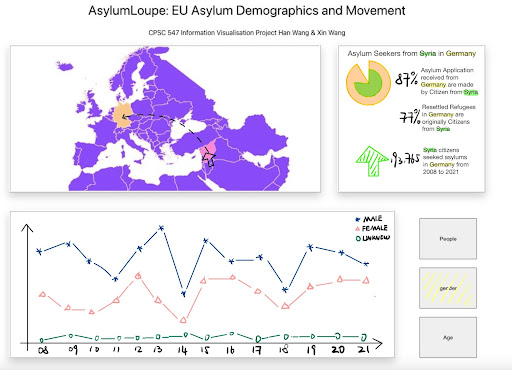
\includegraphics[width=\columnwidth]{fig3}
  \caption{Project Overview Schematic Diagram}
  \label{fig:us1-2}
 \end{figure}

As \autoref{fig:us1-2} shows, take Germany as an example. Assuming we would like to know the movement between the origin countries refugees come from and our targeted destination country Germany, we can select the destination country Germany by clicking inside the country in the EU map. The area of Germany, the destination country, becomes yellow on the map as we click, while the origin country, where the refugees come from, becomes pink. Assuming there are only several origin countries as shown in the same picture. We would like to use the saturation of pink to depict the different levels of the number of arrived refugees. The higher the saturation level is, the more refugees arrive at the destination country from this origin country. To show the flow of refugees more clearly, we may also choose to use a motion map to show the direction better. It will depend on the actual representation effect. If the origin countries are selected, then the second view will depict the detailed information from the origin country to the destination country. Take the combination of Germany and Syria as an example, if the destination country Germany and the origin country Syria are selected, there will be three types of information described, including the current full-year German resettlement of Syrian refugees as a percentage of total applications, the percentage of Syrian refugees resettled in Germany among all refugees resettled in Germany for the current year as a whole, and the total number of Syrian asylum seekers (applications and resettlement) received in Germany from 2008 to 2021.

For the view in \autoref{fig:us1-2}, if the button “gender” is chosen, there will be three line chart describing the number of different gender asylum seekers from 2008 to 2021. Different labels and colors will help users to better differentiate data from other genders. As \autoref{fig:us1-3} shows, if users select the button “age”, the application and resettlement data for asylum seekers divided by four age groups from 2008 to 2021 will be represented in a bar chart format. 

\begin{figure}[tb]
  \centering % avoid the use of \begin{center}...\end{center} and use \centering instead (more compact)
  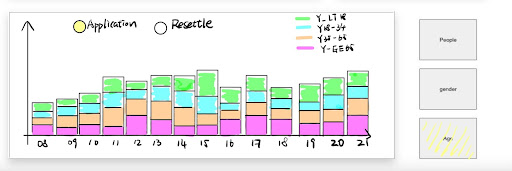
\includegraphics[width=\columnwidth]{fig4}
  \caption{Overview Schematic Diagram for Age Category}
  \label{fig:us1-3}
 \end{figure}

\subsection{User Scenario 2}

\subsubsection{Senario Solution}

For destination EU+ countries where asylum applications are processed, refugee service agencies would like to see a comparison of data for two selected years from 2008 to 2021, to analyze the changes in the number of applications and the trend of the ratio for resettled applicants among all applicants. Although the overview of data from 2008 to 2021 is provided, to make a more customized and clear comparison, refugee service agencies may still need to select two specific years among the 14 to analyze the trend. In that case, the analysis based on the visualized data will help refugee service agencies with their processing speed, work efficiency, and personnel allocation to deal with asylum applications. For example, if the refugee service agencies find out there is an increasing trend in the ratio between applications and resettlements by comparing the yearly application and settlement data, they may need to enhance their efficiency of the asylum application processing by some adjustments to meet the increased needs of asylum applicants. For another example, refugee service agencies can judge whether it is necessary to expand refugee shelters based on the trend of the number of asylum applications flowing from the origin country to the destination country by comparing the data between two selected years.

\subsubsection{Implementation Method}

The other part of the visualization views will be the same as before except for the view under the orient-destination map as \autoref{fig:us2-1} shows. Users can make a comparison for the data between two different years for three types of data including “people”, “gender” and “age” after clicking the “Yearly Comparison” button outside. 

\begin{figure}[tb]
  \centering % avoid the use of \begin{center}...\end{center} and use \centering instead (more compact)
  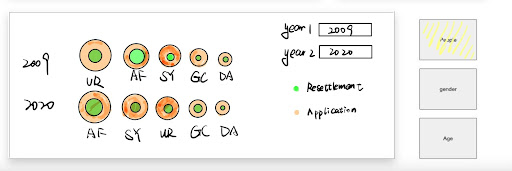
\includegraphics[width=\columnwidth]{fig5}
  \caption{Overview Schematic Diagram for Two Selected Year}
  \label{fig:us2-1}
 \end{figure}

To implement the function of time selection, we have included two time-select menus for users to select different years to make comparisons with. In that case, refugee service agencies are able to determine the trend of refugee movements within the EU over time. 

Besides, this vis also allows the comparison of application and resettlement data between different origin countries where the asylum seekers come from. We use the green color to represent the number of resettled asylum applicants from an origin country. So as the orange color represents the number of applications made from an origin country. The comparison between the number of applications and resettlements for a specific country can be made more intuitively through concentric circles with a certain degree of transparency. When clicking the button “people”, the data will be divided into groups by 5 main origin countries as \autoref{fig:us2-1} shows, and that will be divided into groups by three gender types or four age categories by clicking the button “gender” and “age” respectively. The data will also be sorted based on its quantity among all groups. 


\section{Implementation}
\section{Milestones}
\section{Results}
\section{Discussion and Future Work}
\section{Conclusions}


%% if specified like this the section will be committed in review mode
% \acknowledgments{
% The authors wish to thank A, B, and C. This work was supported in part by
% a grant from XYZ (\# 12345-67890).}

%\bibliographystyle{abbrv}
%\bibliographystyle{abbrv-doi}
%\bibliographystyle{abbrv-doi-narrow}
\bibliographystyle{abbrv-doi-hyperref}
%\bibliographystyle{abbrv-doi-hyperref-narrow}

\bibliography{template}
\end{document}

